\chapter{Implementación}


A la hora de implementar esta nueva arquitectura debemos considerar que, para ejecutarla, hay que crear un entorno, un escenario, real sobre el que hacerlo. O, en su defecto, crear un entorno que simule esas condiciones para trabajar con ella.

Es por ello que antes de trabajar con el modelo de ``Swiftnet'' \cite{swiftnet} tenemos que sentar las bases sobre las que se pueda ejecutar. Así comienza la creación de un entorno Conda.

\section{Conda}

Conda \cite{conda} es un sistema de gestión de entornos con el que creamos el escenario sobre el que vamos a correr ``Swiftnet'' \cite{swiftnet}. Conda permite crear el escenario instalando y gestionando paquetes de uso público ubicados en diferentes ``canales'' del sistema. Simplemente hay que seguir las instrucciones que dan para descargarlos e instalarlos, y poder añadirlos así al escenario sobre el que se esté trabajando.

\begin{figure}[H]
  \centering
  
\includegraphics[width=8cm]{Figuras/Conda.eps}
  \caption{Conda}
\end{figure}

Antes de crear ningún entorno, primero hay que instalar Conda en la máquina que va a procesar el proyecto. Para ello descargamos Miniconda (un instalador de Conda) para Python 2.7 \cite{miniconda_install}. Una vez descargado ya podemos crear entornos Conda.


Para crear el entorno Conda sobre el que trabajar basta con abrir un terminal del sistema operativo y escribir el siguiente comando:

\begin{center}
\textit{conda  create  --name  swiftnet  python=3.7}
\end{center}

En este caso estamos creando un entorno Conda llamado ``swiftnet'' con la versión de Python 3.7 (la necesaria para el modelo de ``Swiftnet'', aunque se admiten versiones superiores  \cite{github_swiftnet}).


Ya tenemos creado el entorno, ahora hace falta añadirle los paquetes necesarios que requiere ``Swiftnet'', indicados en el archivo ``requirements.txt'' \cite{github_swiftnet}. Para instalarlos simplemente seguimos las indicaciones del modelo y usamos este comando:

\begin{center}
\textit{pip install -r requirements.txt}
\end{center}

``Pip'' es otro gestor de paquetes que, junto a Conda, es muy útil a la hora de instalar aquellos paquetes que Conda no posee en sus ``canales'' \cite{pip}.

Con el anterior comando, se instalan una serie de paquetes necesarios para la ejecución del modelo, entre ellos PyTorch \cite{pytorch}, del cual hablaremos más adelante; pero no todos (en nuestro caso). Para que el modelo funcione correctamente hay que instalar los restantes con este comando \cite{conda_sheet}:

\begin{center}
\textit{conda install nombre\_del\_paquete -c nombre\_del\_canal\_en\_el\_que\_se\_encuentra\_el\_paquete}
\end{center}

A continuación enumeramos los paquetes que quedan para poder ejecutar ``Swiftnet'':

\begin{enumerate}
\item opencv \cite{opencv}
\item pytorch torchaudio=0.4.0 cudatoolkit=10.0 \cite{pytorch}
\end{enumerate}

Cabe destacar que ponemos dichos paquetes con estas versiones porque las especificaciones de nuestra máquina lo requerían. Si se quiere reproducir el resultado de este proyecto, puede que no sean las mismas versiones de estos paquetes los que haya que instalar, dependerá de la máquina sobre la que se trabaje.

Una vez instalados dichos paquetes, se sigue el procedimiento marcado por el modelo (se descargan la base de datos de Cityscapes \cite{cityscapes} y una serie de modelos preentrenados para la misma en la carpeta ``weights'' \cite{github_swiftnet}) y se ejecuta desde el directorio en el que éste se encuentra:

\begin{center}
\textit{python eval.py configs\textbackslash{rn18\_single\_scale.py}}
\end{center}

Tras ello, y en nuestro caso particular, se llegarán a dos errores:

\begin{enumerate}
\item No se encuentra el módulo ``lib.cylib''
\item No se encuentra la versión ``GLIBCXX\_3.4.26'' de ``libstdc++'' que se encuentra en el sistema operativo
\end{enumerate}

Pasamos a explicarlos:

\subsection{Error de ``lib.cylib''}

Este error se da porque aún no se ha creado módulo de ``cython'' \cite{cython} necesario para evaluar las métricas del modelo. Se consigue ejecutando el código del archivo ``build.sh'' del modelo en la carpeta ``lib\textbackslash{}'' de éste.

Sin embargo, antes de ejecutarlo conviene modificarlo de la siguiente manera:

\begin{figure}[H]
  \centering
  \includegraphics[width=12cm]{Figuras/cylib.eps}
  \caption{Archivo ``build.sh''}
  \label{fig:cylib}
\end{figure}

Tras hacerlo, lo ejecutamos con el siguiente comando:

\begin{center}
\textit{.\textbackslash{build.sh}}
\end{center}

Si nos sale algún error porque falta algún paquete por instalar, volvemos al comando que utilizamos para instalar paquetes por Conda y los instalamos de forma sencilla.

Como se puede observar en la figura \ref{fig:cylib}, el archivo está en ``Shell Script'' \cite{shell} y a través de éste se crean los archivos ``cylib.so'', ``cylib.cc'' y ``cylib.html''.

Cabe destacar otra observación muy importante en la figura: Hay que modificar las líneas en las que se hace referencia al sistema de archivos propio de la máquina sobre la que se trabaja.

En nuestro caso, tenemos la siguiente ruta seguida de los directorios que se han creado al haber instalado los paquetes previos a la ejecución del modelo:

\begin{center}
\textit{\textbackslash{home}\textbackslash{sergios}\textbackslash{miniconda2}\textbackslash{envs}\textbackslash{swiftnet}}
\end{center}

Es muy importante cambiar esa ruta por la de la máquina sobre la que se trabaje, si no, no puede funcionar; de modo que cuando se instale Conda y se cree el entorno sobre el que se quiere trabajar, hay que tener muy en cuenta dónde se instala para modificarla.

Por otro lado, el resto de la ruta no se cambia, ya que son paquetes comunes a cualquier usuario que intente ejecutar ``Swiftnet'' \cite{swiftnet}.

Por último, puntualizar que la última parte comentada del archivo, que es muy similar a la que hemos modificado hace un momento, sirve para lo mismo pero utilizando Python 3.8. Si se quisiese utilizar este modelo con esa versión de Python habría que descomentarla y comentar la referente a Python 3.7. Lo demás se mantendría como está.

\subsection{Error de ``GLIBCXX''}

Para empezar, ``libstdc++'' \cite{glibcxx} es la implementación de la librería estándar del lenguaje C++ de programación.

Esto quiere decir que para cualquier programa en C++ que use hilos o archivos, por ejemplo, usará esta librería para implementar lo pertinente a estas cosas en las librerías de C++.

Por otro lado tenemos la \ac{ABI} \cite{glibcxx}, la cual sirve para que, por ejemplo, un programa compilado en ``libstdc++'' en 2013 funcione de la misma manera para una nueva versión de ``libstdc++'' en 2021. Cuando se actualiza esa librería y se quiere compilar un programa de una versión anterior, se mantiene la ABI de dicha versión para compilar ese programa.

Sin embargo, cuando se actualiza ``libstdc++'' y se mantiene su ABI, cada función o símbolo de dicha librería obtiene una nueva versión, a la que se le llama mediante un ``linker''.

El ``linker'' enlaza la llamada a una función de la librería con su última versión \cite{glibcxx}.

Para nuestro caso, no encuentra la versión ``GLIBCXX\_3.4.26'' de ``libstdc++'' debido a que el ``linker'' no tiene permisos para acceder a la librería del sistema operativo. Por lo que, cada vez que ejecutemos el modelo, aunque lo intente, no podrá encontrar dicha librería.

Sin embargo, he aquí una razón de uso de los entornos Conda: Cuando se crea un entorno Conda nuevo, éste también adquiere esta librería al venir incluida en uno de los paquetes de instalación predeterminados para la creación del entorno. De este modo obtenemos la versión que requiere ``Swiftnet'' para su ejecución.

Aún así sigue existiendo un problema: el ``linker'' sigue buscando la versión requerida por ``Swiftnet'' en el mismo lugar, de modo que cada vez que se llame a esa librería el ``linker'' seguirá buscando donde siempre y seguiremos igual. La solución reside en hacerle saber al ``linker'' dónde buscar esta nueva versión, y para ello usaremos este comando en la terminal:

\begin{center}
\textit{export LD\_LIBRARY\_PATH=\$LD\_LIBRARY\_PATH:\$HOME\textbackslash{miniconda2}\textbackslash{lib}\textbackslash{}}
\end{center}

No obstante, esta solución sirve siempre y cuando no se cierre la terminal. En el momento en el que se cierre hay que volver a abrir otra y volver a utilizarlo.

Al usarla, conseguimos nuestro objetivo y podemos seguir avanzando en la ejecución del modelo.

\section{PyTorch}

Anteriormente lo hemos mencionado, y a diferencia de otros paquetes de instalación, éste conviene explicarlo, pues es en lo que se basa ``Swiftnet'' para hacer la \ac{SS}.

\begin{figure}[H]
  \centering
  
\includegraphics[width=8cm]{Figuras/PyTorch.eps}
  \caption{PyTorch}
\end{figure}

PyTorch \cite{pytorch} es un framework de Python de ``deep learning'' que permite su utilización en aplicaciones que implementan visión por computador o IA. Está basado en la librería ``Torch'', de ahí que los paquetes que se requieren instalar por Conda tengan el mismo nombre y derivados.

PyTorch trabaja, entre otras cosas, con ``tensores'', que sirven para operar con arrays de n-dimensiones. Este tipo de variables se usan durante todo el modelo de ``Swiftnet'' ya que son las que obtendrán, por ejemplo, la lectura de datos de las imágenes, la información de las clases de las etiquetas (persona, vehículo...).

En esencia, PyTorch posibilita la existencia del modelo de ``Swiftnet''. Si no se utilizase, podríamos utilizar otros como Tensorflow \cite{tensorflow} o Caffe \cite{caffe}, sin embargo, cada uno de estos frameworks está enfocado hacia diferentes aspectos y habría que analizar cuál de ellos podría ser el adecuado para el modelo. 

PyTorch se puede instalar tanto para máquinas con tarjeta gráfica como sin ella, dependiendo de cómo se quiera ejecutar. Generalmente, se suele instalar en máquinas con tarjeta gráfica y por ello se instala, además de los paquetes de ``Torch'', el paquete ``cudatoolkit''. Este paquete interactúa con CUDA \cite {cuda}.

\subsection{CUDA}

CUDA \cite{cuda} es una plataforma desarrollada por NVIDIA para poder trabajar, a nivel de cómputo, con las \ac{GPU}.

Como ya hemos dicho, el paquete ``cudatoolkit'' es necesario para trabajar con PyTorch en máquinas con tarjeta gráfica (\ac{GPU}). Sin embargo, es posible instalarlo y poder ejecutar PyTorch sin la \ac{GPU}, es decir, a través de la \ac{CPU}.

Basta con hacerle saber a PyTorch sobre qué ejecutarlo con la siguiente instrucción:

\begin{center}
\textit{torch.device(`cpu/gpu')}
\end{center}

Escribiendo dicha instrucción en el código que se quiera ejecutar especificando una de las dos opciones que se dan (\ac{CPU} o \ac{GPU}), podemos obligar a PyTorch a que trabaje con una u otra.


En cuanto a términos de rendimiento, es recomendable ,si es posible, que PyTorch trabaje con \ac{GPU} puesto que al hacerlo de la otra forma, la carga de procesos que tendría que soportar la \ac{CPU} sería elevada y conllevaría a que tardase demasiado la ejecución del modelo. Con \ac{GPU}, sin embargo, sería más veloz y podríamos trabajar con mayor soltura al no tener largos tiempos de espera durante la ejecución del modelo.


\section{Swiftnet}

Ya hemos explicado las bases sobre las que se sustenta ``Swiftnet'' (PyTorch y CUDA) y sobre dónde ejecutarlo (entorno Conda), además de explicar y solucionar los errores que pueden ocurrir durante el proceso. A continuación pasamos a explicar el propio modelo y cómo ejecutarlo paso a paso.

\subsection{Cityscapes}

Para la ejecución del modelo tomaremos como referencia la base de datos de Cityscapes \cite{cityscapes}, como viene indicado en la guía de éste \cite{github_swiftnet}, para poder comparar los resultados con los del paper de ``Swiftnet'' \cite{swiftnet}.

Antes de continuar, es recomendable cambiar el nombre de las bases de datos que se han descargado de Cityscapes por nombres más sencillos por comodidad. En nuestro caso, llamamos ``labels'' a la carpeta que contiene las etiquetas de las imágenes (241 MB) y ``rgb'' a la carpeta que contiene las imágenes (11 GB).

Cuando esté descargada la base de datos, vamos a la carpeta referente a las etiquetas (``labels''). Una vez dentro, tenemos que, o bien borrar todos los archivos ``instanceIds'' y ``color'', o bien moverlos en otra carpeta. Esto es porque durante la ejecución del modelo, éste podría confundirse de archivos y coger los que queremos borrar (o mover), y nos interesa que utilice sólo los llamados ``labelIds''.

También aparecen unos archivos con la extensión ``.json'' que es conveniente dejarlos tal y como están.

\subsection{Pycharm}

Para ejecutar ``Swiftnet'' nos hemos ayudado de un \ac{IDE} llamado ``Pycharm'' \cite{pycharm}.

``Pycharm'' nos sirve para poder comprobar la ejecución del modelo paso a paso. De otra manera, si lo hiciéramos desde la terminal, resultaría mucho más difícil saber cómo procesa las imágenes. Se puede descargar de manera muy sencilla.

\subsection{Proceso de Swiftnet}

Una vez tenemos ``Pycharm'' podemos pasar a ejecutar ``Swiftnet'', el cual funciona de la siguiente manera:

\begin{enumerate}
\item En primera instancia, ``Swiftnet'' carga las especificaciones del archivo de configuración ``rn18\_single\_scale.py'' que pasaremos a modificar a continuación.
\item Más adelante, carga la información de las clases de las etiquetas (persona, carretera, vehículo...).
\item A continuación, carga el modelo de \ac{SS} que se va a utilizar con CUDA \cite{cuda}.
\item Por último, evalúa el modelo cargado usando las imágenes del dataset de Cityscapes, la información de las clases, etc... Para evaluarlo sigue los siguientes pasos:

\begin{itemize}
\item Crea una pila para guardar las predicciones que se van a hacer de las imágenes de Cityscapes. Con ``predicciones'' nos referimos a ``imágenes segmentadas por el modelo''.
\item En la pila creada, se colorizarán las etiquetas de las predicciones y se formarán éstas. En esencia, la pila será la encargada de realizar estas funciones además de guardar los resultados en el directorio adecuado
\item Una vez se crea la pila, se crean lotes de imágenes que van a pasar por el modelo para que éste los vaya segmentando, es decir, que vaya etiquetando las imágenes del lote según las clases que detecte.
\item Una vez todo finaliza, se calcula el porcentaje de acierto que ha tenido el modelo con las imágenes reales. De ahí se extraen los datos que aparecen en el paper de ``Swiftnet''.
\end{itemize}   
\end{enumerate}

Sin embargo, si lo ejecutamos siguiendo el comando que nos dice el procedimiento del modelo no funcionará.

Esto es porque antes de ejecutarlo debemos modificar el archivo ``rn18\_single\_scale.py'' de la carpeta ``configs''. En este archivo, hay que cambiar lo siquiente:

\subsection{Archivo rn18\_single\_scale.py}

\begin{enumerate}
\item Modificar dos rutas en las líneas que se detallan:
\begin{itemize}
\item `datasets' en la línea 18
\item `weights\textbackslash{rn18\_single\_scale}\textbackslash{model\_best.pt}' en la línea 70
\end{itemize}

Básicamente hay que modificarlas poniendo la ruta absoluta en cada una de ellas para asegurarnos de que, al ejecutar el modelo, encuentre los archivos de éstas; indicando además en la primera el directorio del dataset de Cityscapes.

\item Añadir la siguiente instrucción en las línea 45 del archivo (opcionalmente se puede añadir en la línea 57, pero sólo si se quisiese entrenar el modelo, cosa que no haremos puesto que no es necesario):

\begin{center}
\textit{RemapLabels(Cityscapes.map\_to\_id, Cityscapes.num\_classes)}
\end{center}

Esta última es de vital importancia para el funcionamiento de ``Swiftnet''. Cuando ejecutamos ``Swiftnet'' y no ponemos esta instrucción, cada vez que analice las etiquetas de una imagen se confundirá.

Esto es porque cuando ``Swiftnet'' obtiene las etiquetas de Cityscapes (``data\textbackslash{cityscapes}\textbackslash{labels.py}''), filtra sólo las que le son necesarias. Cada una de ellas viene identificada por un número (por ejemplo, la clase ``carretera'' tiene asociado el número 7). De este modo, cuando filtra las clases, por cómo accede a ellas para saber cual es cual, obvia estos números y las identifica por el orden en que se han filtrado.

Tomando el ejemplo de la clase ``carretera'': Si esta clase tiene asociado el número 7, y ha sido filtrada en primer lugar, aunque el modelo detecte que en una imagen hay etiquetas de la clase ``carretera'' (con el número 7), para él ``carretera'' tendrá el número 0 por ser la primera clase filtrada.

Con la instrucción anterior evitamos ese tipo de errores.
\end{enumerate}

Por último, debemos modificar un último archivo para poder generar los resultados de ``Swiftnet''

Para que funcione ``Swiftnet'', nos vamos al directorio ``data'' del modelo, y a su vez no dirigimos al que lleva por nombre ``cityscapes'', para modificar el archivo ``cityscapes.py''.

\subsection{Archivo cityscapes.py}

Éste archivo es el responsable de obtener las imágenes de la base de datos de Cityscapes pero si no hacemos los siguientes cambios no cumplirá con lo establecido:

\begin{enumerate}
\item `home = Path.home()' en la línea 5.

Esta instrucción crea una variable llamada ``home'' que contendrá la ruta hacia el directorio homónimo.

\item `self.root = home' en la línea 41.

Inicializamos la variable ``self.root'' con el valor de la variable ``home'' antes creada.

\item `self.images\_dir = self.root \textbackslash{} `Desktop' \textbackslash{} `swiftnet' \textbackslash{} `datasets' \textbackslash{} `Cityscapes' \textbackslash{} `rgb' \textbackslash{} subset' en la línea 42.

Básicamente estamos cambiando la ruta por donde va a obtener las imágenes de Cityscapes.

\item `self.labels\_dir = self.root \textbackslash{} `Desktop' \textbackslash{} `swiftnet' \textbackslash{} `datasets' \textbackslash{} `Cityscapes' \textbackslash{} labels\_dir \textbackslash{} subset' en la línea 43.

Cambiamos la ruta por donde va a obtener las etiquetas de las clases de Cityscapes.

\item `self.images = list(sorted(self.images\_dir.glob(`*\textbackslash{*.png}'))' en la línea 48

Como se puede ver, la instrucción es la misma salvo en el final: Simplemente obtenemos una lista ordenada de archivos ``.png'' de la base de datos de Cityscapes y la guardamos en la variable ``self.images''.
\end{enumerate}

\subsection{Final}

Para concluir, con todo esto ya podemos ejecutar el modelo con la instrucción:

\begin{center}
\textit{python eval.py configs\textbackslash{rn18\_single\_scale.py}}
\end{center}

Si hemos hecho todo bien, obtendremos los mismos resultados que en el paper de ``Swiftnet'' \cite{swiftnet}.

Cuando veamos las imágenes segmentadas, veremos que no están todas las del dataset de Cityscapes; esto es porque hemos ejecutado el modelo para evaluación (``eval.py''), de modo que sólo ha procesado las imágenes del dataset de la subcarpeta ``val''. Se puede modificar para que coja todas, pero en este caso no es necesario.

Sin embargo, nuestro trabajo no lo hemos realizado con la base de datos de Cityscapes, sino con la de $ISA^{2}$ \cite{isa2}. Para hacerlo con esa base de datos simplemente hay que:

\begin{itemize}
\item Cambiar las rutas del dataset de Cityscapes y sustituirlo por $ISA^{2}$ en el archivo ``rn18\_single\_scale.py'' en las líneas que modificamos previamente.
\item Comentar las líneas 77, 79, 82 del archivo ``evaluation\textbackslash{evaluate.py}''
\item Modificar el archivo ``cityscapes.py'' siguiendo las siguientes figuras:

\begin{figure}[H]
  \centering
  \includegraphics[width=16cm]{Figuras/cityscapes.py_1.eps}
  \caption{Archivo ``cityscapes.py'' Parte 1}
\end{figure}

\begin{figure}[H]
  \centering
  \includegraphics[width=16cm]{Figuras/cityscapes.py_2.eps}
  \caption{Archivo ``cityscapes.py'' Parte 2}
\end{figure}

\begin{figure}[H]
  \centering
  \includegraphics[width=8cm]{Figuras/cityscapes.py_3.eps}
  \caption{Archivo ``cityscapes.py'' Parte 3}
  \label{fig:pred.py3}
\end{figure}

\item Por último, modificar la clase ``StorePreds'' del archivo ``prediction.py'' en la carpeta ``evaluation\textbackslash{}'' siguiendo las siguientes figuras:

\begin{figure}[H]
  \centering
  \includegraphics[width=16cm]{Figuras/prediction.py_1.eps}
  \caption{Archivo ``prediction.py'' Parte 1}
\end{figure}

\begin{figure}[H]
  \centering
  \includegraphics[width=16cm]{Figuras/prediction.py_2.eps}
  \caption{Archivo ``prediction.py'' Parte 2}
\end{figure}

\begin{figure}[H]
  \centering
  \includegraphics[width=16cm]{Figuras/prediction.py_3.eps}
  \caption{Archivo ``prediction.py'' Parte 3}
\end{figure}

Hemos modificado de esta manera el archivo ``cityscapes.py'' porque buscábamos que obtuviese las imágenes de manera automática de los subdirectorios de la base de datos de $ISA^{2}$. De la misma forma, los cambios en el archivo ``prediction.py'' persiguen el mismo objetivo: Guardar las imágenes procesadas de manera automática en los subdirectorios correspondientes.

A pesar de que son muchas modificaciones en estos dos últimos archivos, no son necesarias para la ejecución del modelo. En nuestro caso particular lo hemos hecho así por comodidad, pero no imprescindible para que funcione.

Siendo opcionales estas modificaciones, para lograr que el programa se ejecute con la base de datos de $ISA^{2}$ sin que se ``automatice'', basta con observar los mismos archivos para el dataset de Cityscapes y aplicar los cambios que se crean oportunos; ya que, teniéndolos como referencia, se puede ver de forma intuitiva qué partes se han de modificar. Sin embargo, la figura \ref{fig:pred.py3} es obligatoria en cualquier caso.

Cabe destacar que en el archivo ``prediction.py'', siguiendo las figuras, se puede ver la llamada a un método llamado ``savemat''. Éste sirve para guardar las imágenes segmentadas en archivos ``.mat'' que en el siguiente paso utilizaremos, de modo que, aunque no es estrictamente imprescindible, sí es recomendable usarlo puesto que nos resultará mucho más fácil manejar las imágenes segmentadas en los códigos de MatLab \cite{matlab} si están en ese formato.

\end{itemize}

Aquí acaba todo lo pertinente a Swiftnet. Hemos visto cómo ha segmentado las imágenes y el proceso interno que lo hace posible, además de trabajar con dos bases de datos. El siguiente paso es la realización de histogramas de las imágenes segmentadas y su posterior introducción en los sistemas de regresión para estimar la velocidad adecuada. Todo ello se hará en MatLab \cite{matlab}.

\section{Realización de histogramas}

